\documentclass[11pt,compress,t,notes=noshow, xcolor=table]{beamer}
\documentclass[11pt,compress,t,notes=noshow, xcolor=table]{beamer}
\usepackage[]{graphicx}\usepackage[]{color}
% maxwidth is the original width if it is less than linewidth
% otherwise use linewidth (to make sure the graphics do not exceed the margin)
\makeatletter
\def\maxwidth{ %
  \ifdim\Gin@nat@width>\linewidth
    \linewidth
  \else
    \Gin@nat@width
  \fi
}
\makeatother

\definecolor{fgcolor}{rgb}{0.345, 0.345, 0.345}
\newcommand{\hlnum}[1]{\textcolor[rgb]{0.686,0.059,0.569}{#1}}%
\newcommand{\hlstr}[1]{\textcolor[rgb]{0.192,0.494,0.8}{#1}}%
\newcommand{\hlcom}[1]{\textcolor[rgb]{0.678,0.584,0.686}{\textit{#1}}}%
\newcommand{\hlopt}[1]{\textcolor[rgb]{0,0,0}{#1}}%
\newcommand{\hlstd}[1]{\textcolor[rgb]{0.345,0.345,0.345}{#1}}%
\newcommand{\hlkwa}[1]{\textcolor[rgb]{0.161,0.373,0.58}{\textbf{#1}}}%
\newcommand{\hlkwb}[1]{\textcolor[rgb]{0.69,0.353,0.396}{#1}}%
\newcommand{\hlkwc}[1]{\textcolor[rgb]{0.333,0.667,0.333}{#1}}%
\newcommand{\hlkwd}[1]{\textcolor[rgb]{0.737,0.353,0.396}{\textbf{#1}}}%
\let\hlipl\hlkwb

\usepackage{framed}
\makeatletter
\newenvironment{kframe}{%
 \def\at@end@of@kframe{}%
 \ifinner\ifhmode%
  \def\at@end@of@kframe{\end{minipage}}%
  \begin{minipage}{\columnwidth}%
 \fi\fi%
 \def\FrameCommand##1{\hskip\@totalleftmargin \hskip-\fboxsep
 \colorbox{shadecolor}{##1}\hskip-\fboxsep
     % There is no \\@totalrightmargin, so:
     \hskip-\linewidth \hskip-\@totalleftmargin \hskip\columnwidth}%
 \MakeFramed {\advance\hsize-\width
   \@totalleftmargin\z@ \linewidth\hsize
   \@setminipage}}%
 {\par\unskip\endMakeFramed%
 \at@end@of@kframe}
\makeatother

\definecolor{shadecolor}{rgb}{.97, .97, .97}
\definecolor{messagecolor}{rgb}{0, 0, 0}
\definecolor{warningcolor}{rgb}{1, 0, 1}
\definecolor{errorcolor}{rgb}{1, 0, 0}
\newenvironment{knitrout}{}{} % an empty environment to be redefined in TeX

\usepackage{alltt}
\newcommand{\SweaveOpts}[1]{}  % do not interfere with LaTeX
\newcommand{\SweaveInput}[1]{} % because they are not real TeX commands
\newcommand{\Sexpr}[1]{}       % will only be parsed by R
\newcommand{\xmark}{\ding{55}}%


\usepackage[english]{babel}
\usepackage[utf8]{inputenc}

\usepackage{dsfont}
\usepackage{verbatim}
\usepackage{amsmath}
\usepackage{amsfonts}
\usepackage{amssymb}
\usepackage{bm}
\usepackage{csquotes}
\usepackage{multirow}
\usepackage{longtable}
\usepackage{booktabs}
\usepackage{enumerate}
\usepackage[absolute,overlay]{textpos}
\usepackage{psfrag}
\usepackage{algorithm}
\usepackage{algpseudocode}
\usepackage{eqnarray}
\usepackage{arydshln}
\usepackage{tabularx}
\usepackage{placeins}
\usepackage{tikz}
\usepackage{setspace}
\usepackage{colortbl}
\usepackage{mathtools}
\usepackage{wrapfig}
\usepackage{bm}
\usepackage{amsmath}
\usepackage{pifont}

\usetikzlibrary{shapes,arrows,automata,positioning,calc,chains,trees, shadows}
\tikzset{
  %Define standard arrow tip
  >=stealth',
  %Define style for boxes
  punkt/.style={
    rectangle,
    rounded corners,
    draw=black, very thick,
    text width=6.5em,
    minimum height=2em,
    text centered},
  % Define arrow style
  pil/.style={
    ->,
    thick,
    shorten <=2pt,
    shorten >=2pt,}
}

\usepackage{subfig}

% Defines macros and environments
\usepackage{../../style/lmu-lecture}


\let\code=\texttt
\let\proglang=\textsf

\setkeys{Gin}{width=0.9\textwidth}

\setbeamertemplate{frametitle}{\expandafter\uppercase\expandafter\insertframetitle}

\usepackage{bbm}
% basic latex stuff
\newcommand{\pkg}[1]{{\fontseries{b}\selectfont #1}} %fontstyle for R packages
\newcommand{\lz}{\vspace{0.5cm}} %vertical space
\newcommand{\dlz}{\vspace{1cm}} %double vertical space
\newcommand{\oneliner}[1] % Oneliner for important statements
{\begin{block}{}\begin{center}\begin{Large}#1\end{Large}\end{center}\end{block}}


%new environments
\newenvironment{vbframe}  %frame with breaks and verbatim
{
 \begin{frame}[containsverbatim,allowframebreaks]
}
{
\end{frame}
}

\newenvironment{vframe}  %frame with verbatim without breaks (to avoid numbering one slided frames)
{
 \begin{frame}[containsverbatim]
}
{
\end{frame}
}

\newenvironment{blocki}[1]   % itemize block
{
 \begin{block}{#1}\begin{itemize}
}
{
\end{itemize}\end{block}
}

\newenvironment{fragileframe}[2]{  %fragile frame with framebreaks
\begin{frame}[allowframebreaks, fragile, environment = fragileframe]
\frametitle{#1}
#2}
{\end{frame}}


\newcommand{\myframe}[2]{  %short for frame with framebreaks
\begin{frame}[allowframebreaks]
\frametitle{#1}
#2
\end{frame}}

\newcommand{\remark}[1]{
  \textbf{Remark:} #1
}

\newcommand{\citebutton}[2]{%
\NoCaseChange{\resizebox{!}{9pt}{\protect\beamergotobutton{\href{#2}{#1}}}}%
}



\newenvironment{deleteframe}
{
\begingroup
\usebackgroundtemplate{\includegraphics[width=\paperwidth,height=\paperheight]{../style/color/red.png}}
 \begin{frame}
}
{
\end{frame}
\endgroup
}
\newenvironment{simplifyframe}
{
\begingroup
\usebackgroundtemplate{\includegraphics[width=\paperwidth,height=\paperheight]{../style/color/yellow.png}}
 \begin{frame}
}
{
\end{frame}
\endgroup
}\newenvironment{draftframe}
{
\begingroup
\usebackgroundtemplate{\includegraphics[width=\paperwidth,height=\paperheight]{../style/color/green.jpg}}
 \begin{frame}
}
{
\end{frame}
\endgroup
}
% https://tex.stackexchange.com/a/261480: textcolor that works in mathmode
\makeatletter
\renewcommand*{\@textcolor}[3]{%
  \protect\leavevmode
  \begingroup
    \color#1{#2}#3%
  \endgroup
}
\makeatother





% ml - trees, extra trees

\newcommand{\Np}{\mathcal{N}} % (Parent) node N
\newcommand{\Npk}{\Np_k} % node N_k
\newcommand{\Nl}{\Np_1}	% Left node N_1
\newcommand{\Nr}{\Np_2} % Right node N_2
\newcommand{\pikN}[1][k]{\pi_#1^{(\Np)}} % class probability node N
\newcommand{\pikNh}[1][k]{\hat\pi_#1^{(\Np)}} % estimated class probability node N
\newcommand{\pikNlh}[1][k]{\hat\pi_#1^{(\Nl)}} % estimated class probability left node
\newcommand{\pikNrh}[1][k]{\hat\pi_#1^{(\Nr)}} % estimated class probability right node


\newcommand{\titlefigure}{figure/categoryplot-binarysmall.pdf}
\newcommand{\learninggoals}{
\item Know how monotone feature transformations affect the tree
\item Understand how categorical features can be treated effectively while growing a CART
\item Understand how missing values can be treated in a CART}

\title{Introduction to Machine Learning}
% \author{Bernd Bischl, Christoph Molnar, Daniel Schalk, Fabian Scheipl}
\institute{\href{https://compstat-lmu.github.io/lecture_i2ml/}{compstat-lmu.github.io/lecture\_i2ml}}
\date{}

\begin{document}
\lecturechapter{CART: \\
Computational Aspects of Finding Splits}
\lecture{Introduction to Machine Learning}

\sloppy

\begin{vbframe}{Monotone feature transformations}

Monotone transformations of one or several features will neither change the value of the splitting criterion nor the structure of the tree,  only the numerical value of the split point.
\vspace{0.5cm}
\begin{columns}[T]
\column{0.49\textwidth}
Original data
\begin{knitrout}\scriptsize
\definecolor{shadecolor}{rgb}{0.969, 0.969, 0.969}\color{fgcolor}
\begin{tabular}{l|r|r|r|r|r}
\hline
x & 1.0 & 2.0 & 7.0 & 10.0 & 20.0\\
\hline
y & 1.0 & 1.0 & 0.5 & 9.0 & 11.0\\
\hline
\end{tabular}


\end{knitrout}
% FIGURE SOURCE: Use picture created in rsrc/monotone_trafo.R
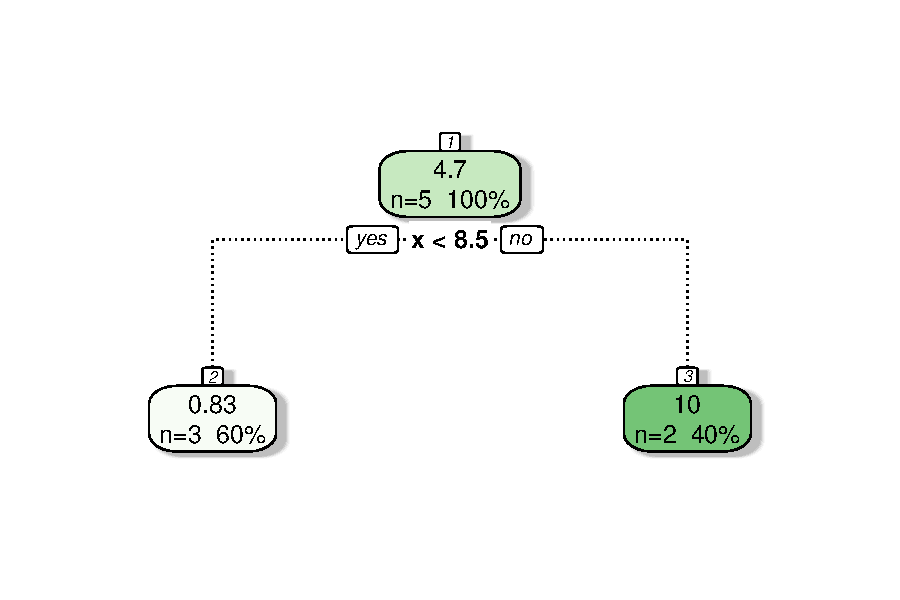
\includegraphics[width = \textwidth]{figure/cart_splitcomp_1}
\column{0.49\textwidth}
Data with log-transformed $x$
\begin{knitrout}\scriptsize
\definecolor{shadecolor}{rgb}{0.969, 0.969, 0.969}\color{fgcolor}
\begin{tabular}{l|r|r|r|r|r}
\hline
log(x) & 0.0 & 0.7 & 1.9 & 2.3 & 3.0\\
\hline
y & 1.0 & 1.0 & 0.5 & 9.0 & 11.0\\
\hline
\end{tabular}


\end{knitrout}
% FIGURE SOURCE: Use picture created in rsrc/monotone_trafo.R
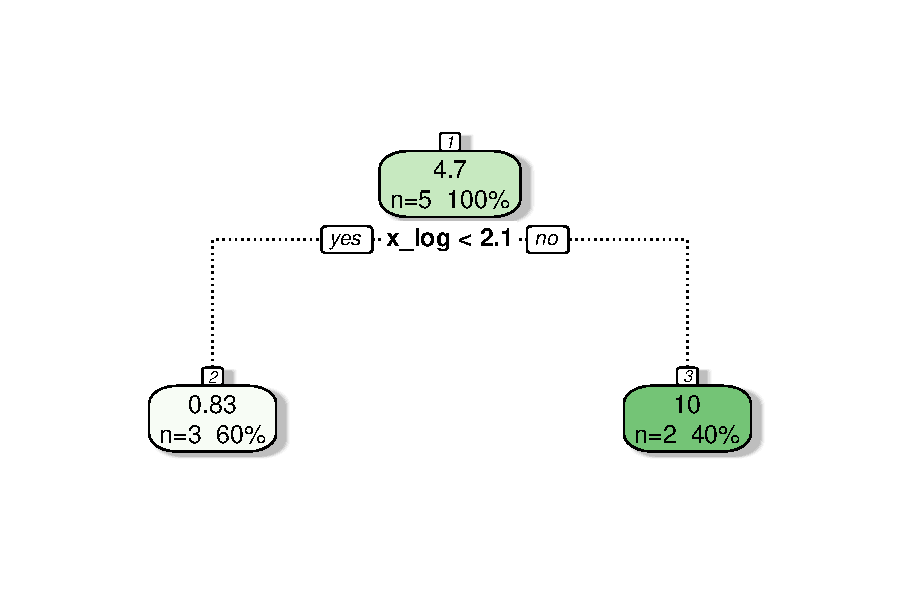
\includegraphics[width = \textwidth]{figure/cart_splitcomp_2}
\end{columns}
\vspace{0.5cm}
\centering
\end{vbframe}

\begin{vbframe}{Categorical Features}
  \begin{itemize}
  \item A split on a categorical feature partitions the feature levels:
    $$x_j \in \{a,b,c\} \leftarrow \Np \rightarrow x_j \in \{d,e\} $$
  \end{itemize}
  \begin{figure}
   \includegraphics[width=0.8\textwidth]{figure/tree-categorical.pdf} 
  \end{figure}
  \end{vbframe}
  
  \begin{vbframe}{Categorical Features}
  \begin{itemize}
  \item A split on a categorical feature partitions the feature levels:
    $$x_j \in \{a,b,c\} \leftarrow \Np \rightarrow x_j \in \{d,e\} $$
  \item For a feature with $m$ levels,
  there are about $2^m$ different possible partitions of the $m$ values into two groups\\ ($2^{m-1} - 1$ because of symmetry and empty groups).
  \item Searching over all these becomes prohibitive for large values of $m$.
  \item For regression with L2 loss and for binary classification, we can define clever shortcuts.
  \end{itemize}

  \end{vbframe}
  
  \begin{frame}{Categorical Features}

For $0-1$ responses, in each node:
  \begin{enumerate}
  \item Calculate the proportion of $1$-outcomes for each category of the feature in $\Np$.

  \end{enumerate}
  \begin{columns}
  \begin{column}{0.33\textwidth}
  \begin{figure}
  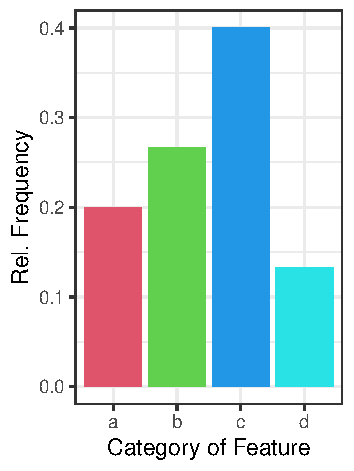
\includegraphics[width=0.8\textwidth]{figure/categoryplot-binary1.pdf} 
  \end{figure}
  \end{column}
  \begin{column}{0.33\textwidth}
  \lz
  \end{column}
  \begin{column}{0.33\textwidth}
  \lz
  \end{column}
  \end{columns}

\end{frame}

  \begin{frame}[noframenumbering]{Categorical Features}

For $0-1$ responses, in each node:
  \begin{enumerate}
  \item Calculate the proportion of $1$-outcomes for each category of the feature in $\Np$.
  \item Sort the categories according to these proportions.
  \end{enumerate}
  \begin{columns}
  \begin{column}{0.33\textwidth}
  \begin{figure}
  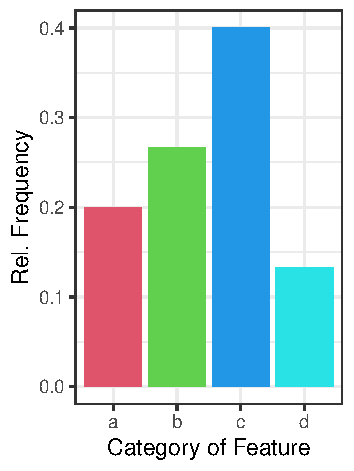
\includegraphics[width=0.8\textwidth]{figure/categoryplot-binary1.pdf} 
  \end{figure}
  \end{column}
  \begin{column}{0.33\textwidth}
  \begin{figure}
  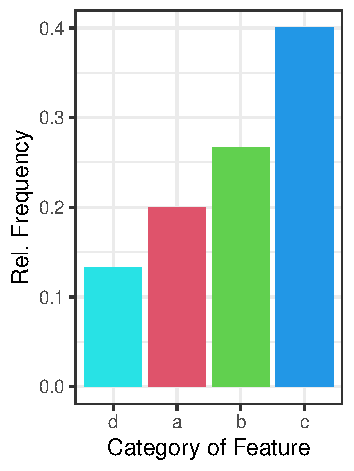
\includegraphics[width=0.8\textwidth]{figure/categoryplot-binary2.pdf} 
  \end{figure}
  \end{column}
  \begin{column}{0.33\textwidth}
  \end{column}
  \end{columns}

\end{frame}

  \begin{frame}[noframenumbering]{Categorical Features}

For $0-1$ responses, in each node:
  \begin{enumerate}
  \item Calculate the proportion of $1$-outcomes for each category of the feature in $\Np$.
  \item Sort the categories according to these proportions.
  \item The feature can then be treated as if it was ordinal, so we only have to investigate at most $m-1$ splits.
  \end{enumerate}
  \begin{columns}
  \begin{column}{0.33\textwidth}
  \begin{figure}
  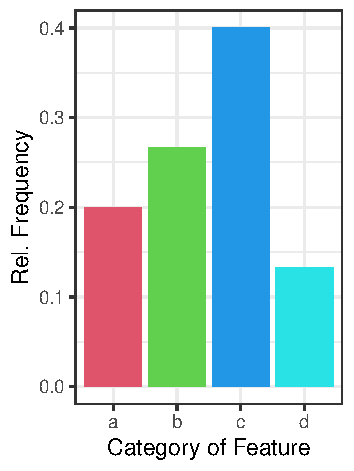
\includegraphics[width=0.8\textwidth]{figure/categoryplot-binary1.pdf} 
  \end{figure}
  \end{column}
  \begin{column}{0.33\textwidth}
  \begin{figure}
  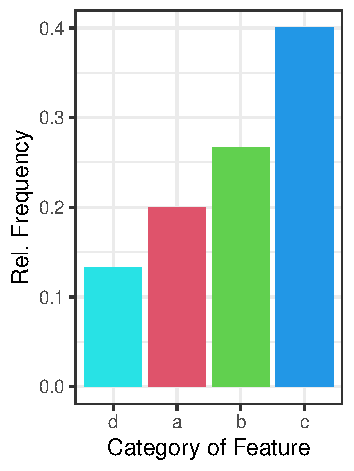
\includegraphics[width=0.8\textwidth]{figure/categoryplot-binary2.pdf} 
  \end{figure}
  \end{column}
  \begin{column}{0.33\textwidth}
  \begin{figure}
  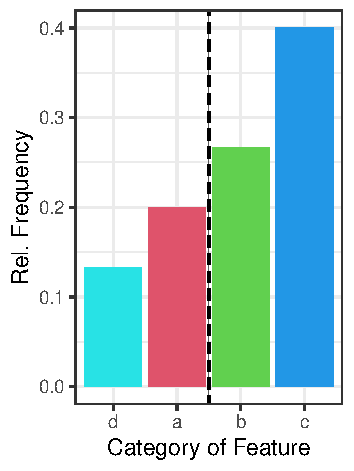
\includegraphics[width=0.8\textwidth]{figure/categoryplot-binary3.pdf} 
  \end{figure}
  \end{column}
  \end{columns}

\end{frame}


\begin{vbframe}{Categorical Features}

  \begin{itemize}
  \item This procedure finds the optimal split.
  \item This result also holds for regression trees (with L2 loss) if the levels of the feature are ordered by increasing mean of the target
  \item The proofs are not trivial and can be found here:
    \begin{itemize}
    \item for 0-1 responses:
      \begin{itemize}
      \item \citebutton{Breiman, 1984, Chapter 4}{https://www.taylorfrancis.com/books/mono/10.1201/9781315139470/classification-regression-trees-leo-breiman}
      \item  \citebutton{Ripley, 1996, pp. 213 et seqq.}{https://www.cambridge.org/core/books/pattern-recognition-and-neural-networks/4E038249C9BAA06C8F4EE6F044D09C5C}
      \end{itemize}
    \item for continuous responses:
      \begin{itemize}
      \item \citebutton{Fisher, 1958}{http://csiss.ncgia.ucsb.edu/SPACE/workshops/2004/SAC/files/fisher.pdf}
      \end{itemize}
    \end{itemize}
  \item There are only heuristics for the multiclass case \citebutton{Wright and König, 2019}{https://www.ncbi.nlm.nih.gov/pmc/articles/PMC6368971/}
  %\item The Algorithm prefers categorical variables with a large value
  %of categories $Q$
  \end{itemize}

\end{vbframe}

\begin{vbframe}{Categorical Features}

For continuous responses, in each node:
  \begin{enumerate}
  \item Calculate the mean of the outcome in each category
  \item Sort the categories by increasing mean of the outcome
  \end{enumerate}

  \begin{columns}
  \begin{column}{0.33\textwidth}
  \begin{figure}
  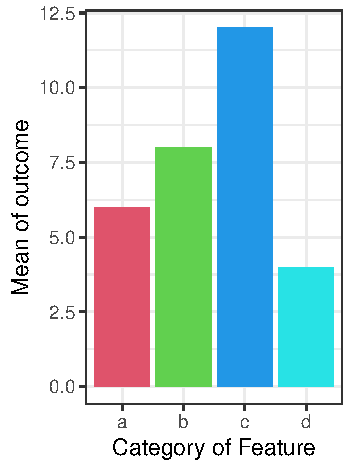
\includegraphics[width=0.8\textwidth]{figure/categoryplot-cont1.pdf} 
  \end{figure}
  \end{column}
  \begin{column}{0.33\textwidth}
  \begin{figure}
  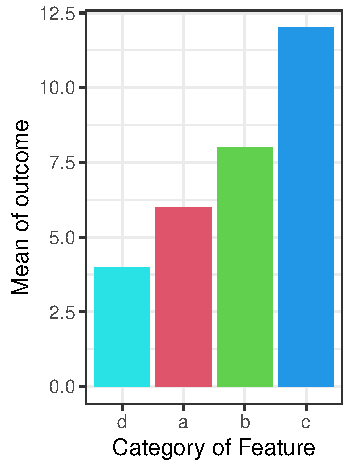
\includegraphics[width=0.8\textwidth]{figure/categoryplot-cont2.pdf} 
  \end{figure}
  \end{column}
  \begin{column}{0.33\textwidth}
  \begin{figure}
  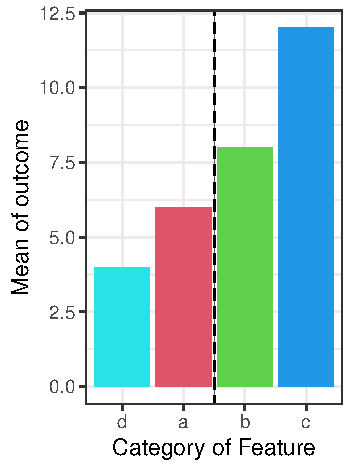
\includegraphics[width=0.8\textwidth]{figure/categoryplot-cont3.pdf} 
  \end{figure}
  \end{column}
  \end{columns}


\end{vbframe}

\begin{vbframe}{Missing feature values}
  \begin{itemize}
    \item When splits are evaluated, only observations for which the used feature is not missing are used. (This can actually bias splits towards using features with lots of missing values.) 
  \item \textbf{Surrogate splits} can deal with missing values during prediction.
  \item Surrogate splits are created during training. They define replacement splitting rules, using a different feature, that result in almost the same child nodes as the original split.
   \item When observations are passed down the tree, % (in training or prediction), 
   and the feature value used in a split is missing, we use the surrogate split instead to decide to which child the data should be assigned. 
  \end{itemize}
\end{vbframe}

\begin{vbframe}{Surrogate Splits}
\begin{itemize}
\item Each surrogate split is a decision stump that tries to learn the actual splitting rule
\item Consider this tree with the primary split w.r.t. \texttt{Sepal.Length} where we perform binary classification (\texttt{setosa} vs. \texttt{virginica}):
\begin{figure}
\includegraphics[width=0.75\textwidth]{figure/tree-binary.pdf} 
\end{figure}
\item Our surrogate split should optimize a splitting criterion w.r.t. \texttt{Sepal.Length < 5.8}
\end{itemize}



\end{vbframe}

\begin{vbframe}{Surrogate Splits}
\begin{itemize}
\item Consider this subsample of the data used to fit the tree:
\begin{table}[ht]
\tiny
\centering
\begin{tabular}{rrrrrll}
  \hline
 & Sepal.Length & ... & Petal.Width & Species & Sepal.Length $<$ 5.8 \\ 
  \hline
1 & 5.10 & ... & 0.20 & setosa & TRUE \\ 
  4 & 4.60 & ... & 0.20 & setosa & TRUE \\ 
  9 & 4.40 & ... & 0.20 & setosa & TRUE \\ 
  15 & 5.80 & ... & 0.20 & setosa & FALSE \\ 
  18 & 5.10 & ... & 0.30 & setosa & TRUE \\ 
  52 & 5.80 & ... & 1.90 & virginica & FALSE \\ 
  57 & 4.90 & ... & 1.70 & virginica & TRUE \\ 
  62 & 6.40 & ... & 1.90 & virginica & FALSE \\ 
  77 & 6.20 & ... & 1.80 & virginica & FALSE \\ 
  99 & 6.20 & ... & 2.30 & virginica & FALSE \\ 
   \hline
\end{tabular}
\end{table}
\item Add column that indicates whether \texttt{Sepal.Length < 5.8}
%\item As this splitting rule is very good, we will have many instances where \texttt{Sepal.Length < 5.8} is \texttt{TRUE} and \texttt{Species} is \texttt{setosa}
\item Fit tree of depth 1 using all features but \texttt{Sepal.Length} %used 
to derive a split that explains 
\texttt{Sepal.Length < 5.8} best $\Rightarrow$ surrogate split
\item Typically, software stores the best and a few more surrogate splits
%\item A good surrogate tries to mimic the primary split this way

\end{itemize}


\end{vbframe}


\endlecture
\end{document}
